\section{Introduction}
%(2 pages)}
\label{sec:intro}

\leanparagraph{Motivation}
Recent advances in information extraction have led to
huge graph-structured knowledge bases (KBs) also known as knowledge graphs (KGs) such as NELL \cite{nell}, DBpedia \cite{dbpedia}, YAGO \cite{yago} and Wikidata \cite{wikidata}. These KGs contain millions or billions of relational facts in the form of subject-predicate-object (SPO) triples, e.g., $\tuple{\mi{clara\;marriedTo\;dave}}$ or $\tuple{\mi{dave\;isA\;researcher}}$. Such triples can be straightforwardly represented by means of positive unary and binary first-order logic facts, e.g. $\mi{marriedTo(clara,dave)}$ and $\mi{researcher(dave)}$.

An important task over KGs is rule learning, which is relevant for a variety of applications ranging from knowledge graph curation (completion, error detection) \cite{DBLP:journals/semweb/Paulheim17} to data mining and semantic culturomics. Rules over KGs are of the form $\mi{head \leftarrow body}$, where $\mi{head}$ is a binary atom and $\mi{body}$ is a conjunction of (possibly negated) binary and unary atoms. 

Traditionally, rule induction has been studied in the context of relational data mining in databases (see e.g., \cite{DBLP:books/daglib/0021868} for overview), and has recently been adapted to KGs (e.g., \cite{amie,op,rdf2rules}). The methods from this area can be used to identify prominent patterns from KGs, such as \emph{``Married people live in the same
place''}, and cast them in the form of Horn rules, such as:
$\mi{r_1:\;}\mi{livesIn(Y,Z)}\leftarrow \mi{marriedTo(X,Y),livesIn(X,Z)}$. 

For the KG curation, this has two-fold benefits. First, since KGs operate under the Open World
Assumption (OWA) (i.e., absent facts are treated as unknown rather than false),
the rules can be used to derive additional facts such as missing living places. % For example, applying the rule
% $\mi{r_1}$ mined from the graph in Figure~\ref{rdf}, the missing living places of Dave and Lucy can be deduced based on the data about their spouses.
Second, rules can be used to eliminate erroneous facts in KGs. For example, assuming that $\mi{livesIn}$ is a functional relation, % Amsterdam as a 
a living place of a person could be questioned if it differs from the spouse's.

When rules are automatically learned, statistical measures like support, confidence and their variations are used to assess the rules' quality. Most notably, the confidence of a rule is the fraction of facts predicted by the rule that are indeed in the KG. However, this is a meaningful measure for rule quality only when the KG is reasonably complete. For rules learned from incomplete KGs, confidence and other measures may be misleading, as they do not reflect the patterns in the missing facts. This might lead to the extraction of erroneous rules from incomplete and biased KGs. For example, a KG that knows a lot of information about families of popular scientists but lacks data in other domains, would yield a heavily biased rule $\mi{r_1':hasChild(X,Y)\leftarrow worksAt(X,Z), educated(Y,Z)}$, stating that workers of certain institutions often have children among the people educated there, as this is frequently the case for scientific families. 

To address this issue, several rule measures that are specifically tailored towards incomplete KGs have been proposed \cite{amie,DBLP:conf/www/ZupancD18} (see \cite{metrics-summary,Azevedo2007} for an overview of other measures). 
Along with KGs themselves, additional background knowledge could be used for better rule assessment. As proposed in \cite{carl} this includes metadata about the concrete numbers of facts of certain types that hold in the real world (e.g., \emph{``Einstein has 3 children''}) automatically extracted from Web resources using techniques like  \cite{paramita-acl-2017}. Other types of background knowledge comprise description logic ontologies, e.g., \cite{d2016ontology} or more general hybrid theories, e.g., \cite{DBLP:journals/tplp/Lisi10,DBLP:journals/tplp/JozefowskaLL10}.

\begin{figure}[t]
\centering
\begin{tikzpicture}[->,>=stealth',auto,node distance=3cm,
  thick,main node/.style={font=\bfseries}]

  \node[main node] (1) {brad};
  \node[main node] (2) [right=2.5cm of 1] {ann};
  \node[main node] (3) [right=3cm of 2] {john};
  \node[main node] (4) [right=2.5cm of 3] {kate};  
  \node[main node] (5) [below right=1cm and 0.5cm of 1] {berlin};  
  \node[main node] (11) [right=1.5cm of 5] {researcher};  
  \node[main node] (6) [above right=0.3cm and 1.5cm of 5] {metropolitan};  
  \node[main node] (7) [right=5cm of 5] {chicago};  
  \node[main node] (9) [below=2.3cm of 1] {bob};  
  \node[main node] (10) [right=2.5cm of 9] {alice};  
  \node[main node] (12) [right=1.6cm of 10] {dave};  
  \node[main node] (8) [right=2.5cm of 12] {clara};  
  \node[main node] (13) [right=6.5cm of 10] {li};  
  \node[main node] (14) [below=1.3cm of 9] {artist};  
  \node[main node] (15) [right=2.4cm of 14] {mat};  
  \node[main node] (17) [right=3cm of 15] {sue};  
  \node[main node] (18) [right=2.5cm of 17] {beijing};  
  \node[main node] (19) [below right=2.7cm and 0.7cm of 1] {lucy};  
  \node[main node] (16) [below right=0.5 and 1.6cm of 10] {amsterdam};  
  
  \path[every node/.style={color=teal,fill=white,font=\small}]
    (1) edge node [right=-23pt] {marriedTo} (2)
    (2) edge node [right=-25pt] {hasBrother} (3)
    (3) edge node [right=-23pt] {marriedTo} (4)
    (9) edge node [right=-23pt] {marriedTo} (10)
    (8) edge node [right=-20pt] {marriedTo} (12)
    (15) edge node [right=-23pt] {marriedTo} (19)
    (17) edge node [right=-23pt] {marriedTo} (13)
    (1) edge node [right=-15pt] {livesIn} (5)    
    (2) edge node [right=-15pt] {livesIn} (5)
    (3) edge node [right=-15pt] {livesIn} (7)    
    (4) edge node [right=-15pt] {livesIn} (7)
    (8) edge node [right=-13pt] {livesIn} (7)    
    (9) edge node [right=-15pt] {livesIn} (5)
    (10) edge node [right=-17pt] {livesIn} (16)    
    (15) edge node [right=-18pt] {livesIn} (16)
    (13) edge node [right=-15pt] {livesIn} (18)    
    (17) edge node [right=-18pt] {livesIn} (18)
    (5) edge node [right=-8pt] {isA} (6)
    (7) edge node [right=-8pt] {isA} (6)    
    (10) edge node [right=-8pt] {isA} (11)
    (12) edge node [right=-8pt] {isA} (11)    
    (9) edge node [right=-8pt] {isA} (14)
    (15) edge node [right=-8pt] {isA} (14)    
    (4) edge node [right=-15pt] {hasFriend} (13)
             ;
\end{tikzpicture}
\caption{Rule mining for KG completion and KG cleaning.}
\label{rdf}
\end{figure}
%\begin{figure}[t]
%\begin{center}
%\begin{subfigure}[b]{0.75\textwidth}
%    \centering
%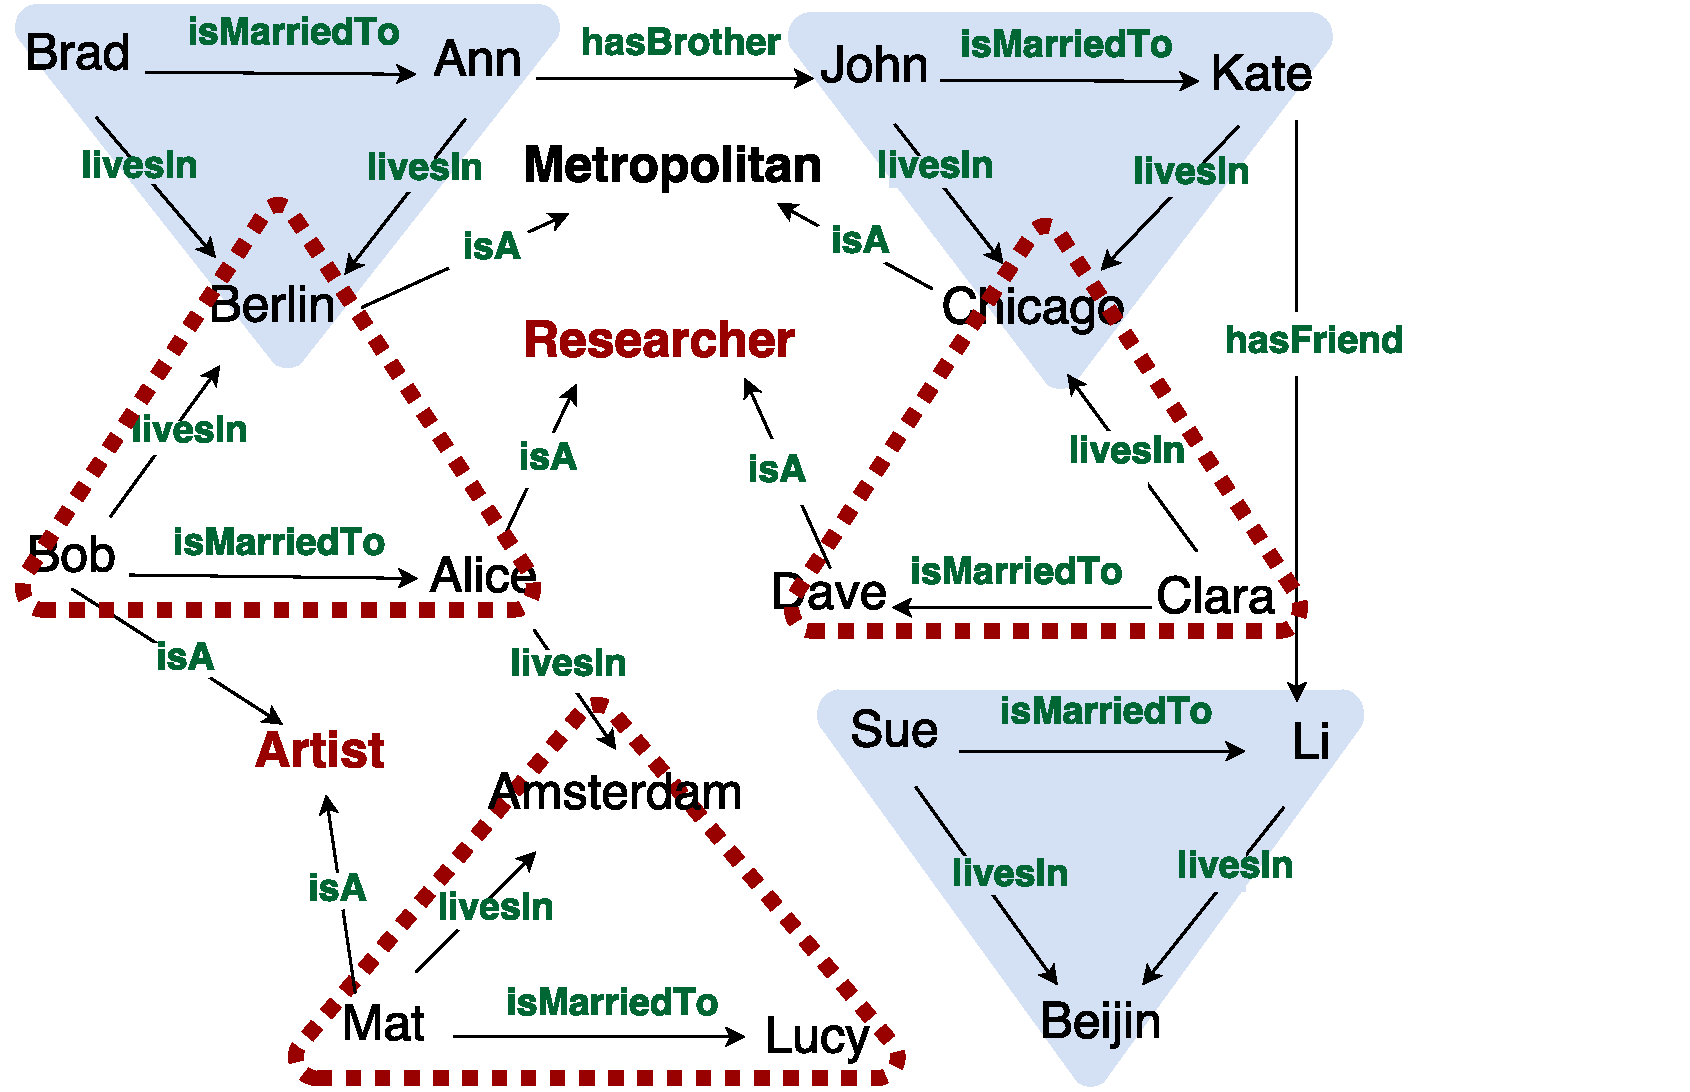
\includegraphics[width=0.7\textwidth]{figures/kg_extended}
%\caption{Rule mining for KG completion and KG cleaning}
%\label{rdf}
%\end{subfigure}
%\begin{subfigure}[b]{0.24\textwidth}
%\scriptsize
%\renewcommand*{\arraystretch}{0.95}
%\begin{tabular}{|l|l|l|l|l|l|l|l|l|}
%\hline
%&  \rot{$\mi{bornInUS}$} &\rot{$\mi{livesInUS}$}&
%\rot{$\mi{stateless}$}&\rot{$\mi{immigrant}$}&\rot{$\mi{singer}$}&\rot{$\mi{poet}$}&\rot{$\mi{hasUSPass}$}\\ \hline
%$\mi{p1}$ & $\checkmark$ &$\checkmark$ &&&$\checkmark$&&$\checkmark$ \\ \hline
%$\mi{p2}$ & $\checkmark$ &$\checkmark$ &&&&&$\checkmark$ \\ \hline
%$\mi{p3}$ & $\checkmark$ &$\checkmark$ &&&$\checkmark$&$\checkmark$&$\checkmark$ \\ \hline
%$\mi{p4}$ & $\checkmark$ &$\checkmark$ &&&&&$\checkmark$ \\ \hline
%$\mi{p5}$ & $\checkmark$ &$\checkmark$ &$\checkmark$&&&& \\ \hline
%$\mi{p6}$ & $\checkmark$ & &$\checkmark$&&&& \\ \hline
%$\mi{p7}$ & $\checkmark$ & &$\checkmark$&&&& \\ \hline
%$\mi{p8}$ & $\checkmark$ & &$\checkmark$&$\checkmark$&&& \\ \hline
%$\mi{p9}$ & $\checkmark$ & &&$\checkmark$&&$\checkmark$& \\ \hline
%$\mi{p10}$ & $\checkmark$ & &&$\checkmark$&$\checkmark$&$\checkmark$& \\ \hline
%$\mi{p11}$ & $\checkmark$ & &&&$\checkmark$&$\checkmark$&$\checkmark$ \\ \hline
%\end{tabular}
%\smallskip
%\caption{US inhabitants KG}
%\label{tab:im}
%\end{subfigure}
%\caption{Examples of Knowledge Graphs}
%\end{center}
%\end{figure}

Even when meaningful, Horn rules, where all predicates in the rule's body are positive such as $\mi{r_1}$ might not always be sufficiently expressive to capture KG patterns accurately, as they cannot handle exceptions, which often appear in practice. 
For instance, application of $\mi{r_1}$ mined from the KG in Figure~\ref{rdf} results in the facts $\mi{livesIn(alice,berlin)}$, $\mi{livesIn(dave,chicago)}$ and $\mi{livesIn(lucy,amsterdam)}$. Observe that the first two facts might be suspected to be wrong. Indeed, both $\mi{alice}$ and $\mi{dave}$ are researchers, and the rule $\mi{r_1}$ could be suspected to have researcher as a potential exception resulting in its more accurate version given as $\mi{r_2:\;}\mi{livesIn(Y,Z)}\leftarrow \mi{marriedTo(X,Y),livesIn(X,Z), not\;researcher(Y)}$.
Exception handling has been faced in inductive logic programming (ILP) by learning nonmonotonic logic programs, i.e., programs with negations from databases (e.g., \cite{DBLP:conf/ijcai/InoueK97,DBLP:journals/tocl/Sakama05,XHAIL}), and recently also studied in the context of KGs \cite{gad2016,rumis}.


The aim of this article is to survey the current research on rule learning from knowledge graphs. We present and discuss different techniques with the roots in inductive logic programming and relational data mining as well as their interrelation and applications for KGs. 

\leanparagraph{Tutorial Overview}
\thi{Could you fix this? Dr.Daria}
In Section~\ref{sec:kgs} we start by briefly introducing knowledge graphs. We then provide necessary preliminaries on rule-based deductive reasoning over KGs and discuss the tasks within the area of inductice logic programming in Section~\ref{sec:reasoning}. Section~\ref{sec:rules_kg_completion} %presents an overview of rule learning tasks that can be performed on KGs and 
describes recent research progress in the context of Horn rule induction for KG completion. We present techniques for nonmonotonic rule extraction in Section~\ref{sec:nmrulelearn}. Finally, in Section~\ref{sec:disc} we conclude the article with an outlook discussion, where we identify a number of promising directions for future work.

